\lab{Applications}{Balanced Trees}{Balanced Trees}
\label{lab:btrees}

Trees are very versatile structures.  
Their worst case complexity of $O(\log n)$ for inserting, deleting, and searching make them an attractive option when working with lots of data.
In most cases, a simple binary search tree is sufficient.
However, there are cases when we lose all the benefits of a binary search tree.
One example is adding already sorted or nearly sorted data to a binary search tree.
This results in a degenerate BST that performs no better than a linked list!
Another problem is adding more levels to the tree than is necessary.
The more levels a tree has, the less performant it becomes.  If we could somehow fill a level or make it as close to full as possible, we can minimize the number of levels a a search tree has.

\begin{problem}
Write methods to determine the number of levels a tree has and how full each level is.  Look at breadth first search for inspiration on how to accomplish this.
\end{problem}

\section*{Balancing Trees}
There have been a variety of attempts at optimizing the structure of a binary tree.
The method that we will describe in depth is and AVL balanced tree.
AVL trees use the strictest definition of balance.
Another commonly used balanced binary tree is a red-black tree.  AVL trees optimize frequent lookups while red-black trees optimize insertion/deletion performance.
Red-black trees color nodes red or black and check for imbalance based on colors.  For example, a subtree is unbalanced if a red node has a red child.
AVL trees determine balance by comparing the height of right and  left subtrees.
The height of a node is the length of the path from a node to its deepest leaf node (the nodes at the base of the tree).
The height of a subtree is length of the path from a node to the deepest leaf node of that subtree.
For every node in an AVL tree, if the difference of height between the left and right subtrees is more than $\pm 1$ levels, then the tree is said to be \emph{out of balance}.  We can restore balance to the entire tree by balancing the nodes where the subtrees are out of balance.
There are four ways a tree can be unbalanced in an AVL tree.

\subsection*{Left-Left and Right-Right}
\begin{figure}[h]
\begin{subfigure}[b]{.49\textwidth}
    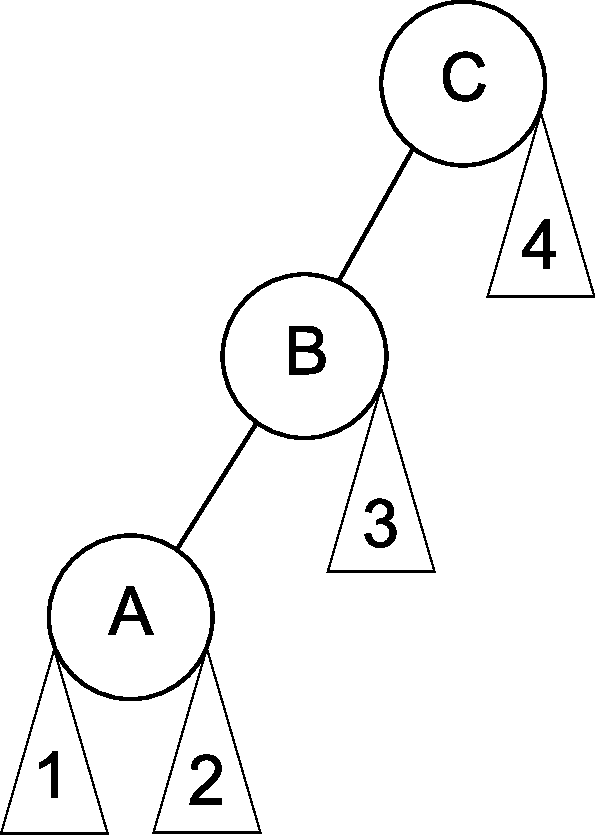
\includegraphics[width=.75\textwidth]{left_left.pdf}
\end{subfigure}
\begin{subfigure}[b]{.49\textwidth}
    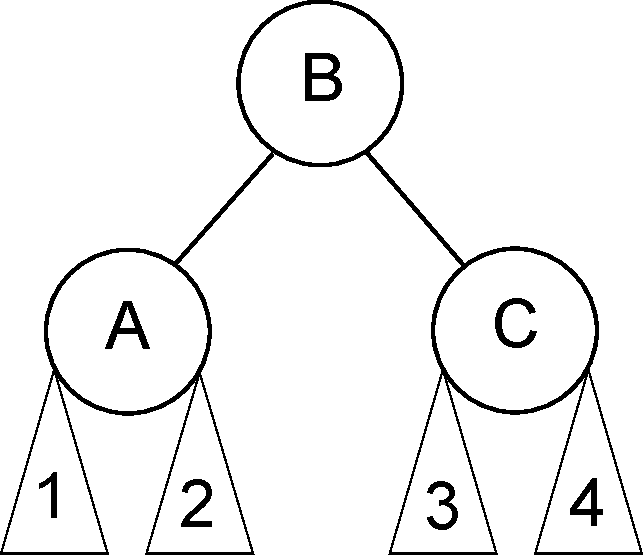
\includegraphics[width=.75\textwidth]{balanced.pdf}
\end{subfigure}
\end{figure}

One of the primary cases, this imbalance can solved by a single rotation.
This will rotate the tree so that node B is the new root of the tree.
Node C becomes a child node of B and the right subtree of node becomes a left subtree of node C.
This preserves the ordered property of the tree.

\begin{figure}[h]
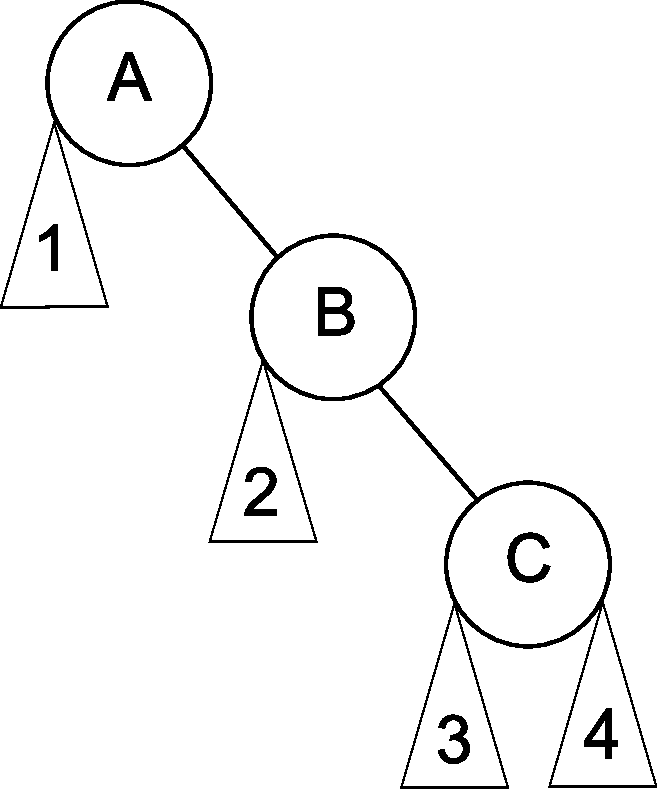
\includegraphics[width=.33\textwidth]{right_right.pdf}
\caption{The mirror image of the Left-Left case.}
\end{figure}

\subsection*{Left-Right and Right-Left}
\begin{figure}[h]
\begin{subfigure}[b]{.49\textwidth}
    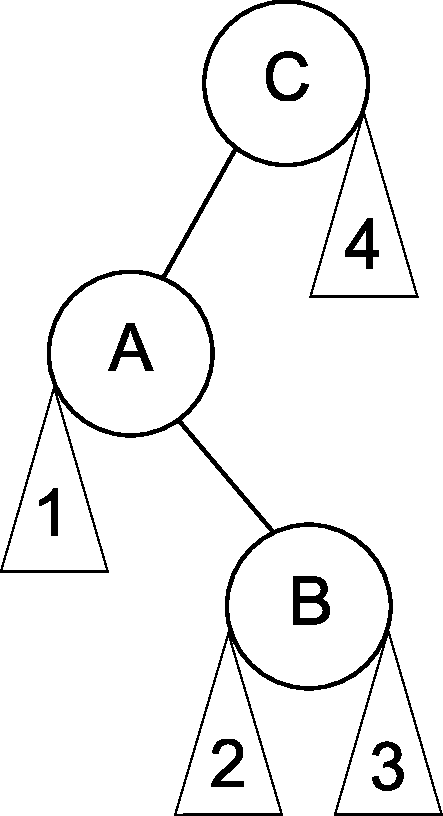
\includegraphics[width=.75\textwidth]{left_right.pdf}
\end{subfigure}
\begin{subfigure}[b]{.49\textwidth}
    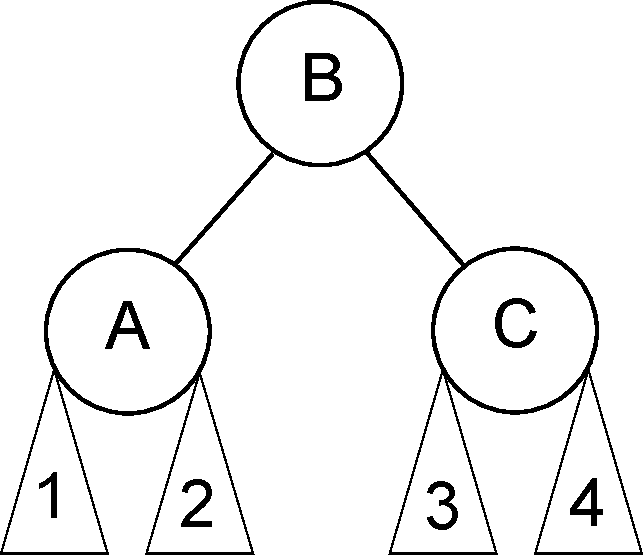
\includegraphics[width=.75\textwidth]{balanced.pdf}
\end{subfigure}
\end{figure}

These cases are a little more complex.
Two rotations must be performed to remedy the imbalance.
Node C is out of balance.
We first need rotate node B to be the parent of node A.
The left subtree of node B becomes the right subtree of node A.
Now we have to do a right rotate, moving node B to be the new root.
Node C becomes a child of node B and the the right subtree of B becomes the left subtree of node C.

\begin{figure}[h]
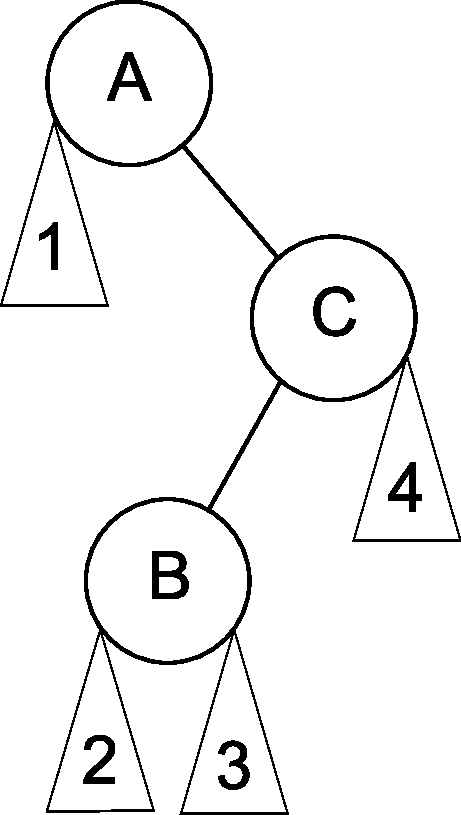
\includegraphics[width=.33\textwidth]{right_left.pdf}
\caption{The mirror image of the Left-Right case.}
\end{figure}

\begin{problem}
Subclass the BST from lab \ref{lab:Python_DataStructures} and add methods for balancing the BST.
You will also need to override the insert and remove methods from the BST because an AVL tree must be re-balanced on each insert or removal.
\end{problem}

\section*{Balanced Trees}
An AVL tree is an improvement over the ordinary BST because the tree is kept in an optimal shape.
There is, however, an even better improvement that can be made.
B-Trees are a very efficient form of balanced tree.
What makes them efficient?  B-Trees relax the requirement of only two children per node.
Balancing a B-Tree is also much simpler than balancing an AVL tree.
Balance is achieved when all leaf nodes are at the same depth.
Instead of using rotations to balance the tree, the B-Tree uses splitting and joining of nodes to maintain balance.

\subsection*{Structure of a B-Tree}
B-Trees are efficient due to their extreme branching.  It is common for B-Trees to hundreds, maybe even thousands of branches.
This extreme branching per node reduces the overall height of the tree considerably.
B-Trees of order $n$ satisfies the following properties:
\footnote{Knuth, Donald. \emph{The Art of Computer Programming: Sorting and Searching (Volume 3, $2^{nd}$ edition)}. New Jersey: Addison-Wesley, 1998. pp 483.}
\begin{enumerate}
\item Every node has at most $n$ children.
\item Every node, except for the root and the leaves, has at least $n/2$ children.
\item The root has at least 2 children (unless it is a leaf).
\item \label{enum:infoleaf} All leaves appear on the same level, and carry no information.
\item A nonleaf node with $n$ children contains $n-1$ keys.
\end{enumerate}
Some implementations modify requirement \ref{enum:infoleaf} so that all information is stored in only the leaf nodes.  In Knuth's original definition, the leaf nodes have references to the information we are storing rather than containing it directly.

The number of keys that a single B-Tree can hold grows exponentially with each new level of the tree.  A B-Tree of depth, $d$, and order $n$ (meaning each node can have at most $n$ children) can store a maximum of $n^{d} - 1$ keys.  For example, a B-Tree of order 100 and depth 3 can store 999999 keys.  Adding a new level increases the total capacity one hundred fold, or 99999999 keys!
In a B+Tree, the actual data of the tree is stored only in the bottom most nodes, or leaf nodes.  All other nodes in the tree are index nodes.

Unlike binary tree, B-Trees are built from the bottom up (starting with a single leaf node).  As more leaves are added, the root changes from a leaf node to an index node.  

\begin{problem}
Verify that the maximum number of keys that a B-Tree of order $n$ and depth $d$ is $n^{d}-1$.
What is the maximum number of keys an AVL tree of depth $d$ can store?

Suppose a disk seek time is $.15$ms and we have an AVL tree and B-Tree stored on disk.  The B-Tree is order 50.
Predict the time required to access a leaf of the AVL tree.  The B-Tree?
It is for this reason that B-Trees are great for on-disk storage.  B-Trees are used in a variety of settings including databases and filesystems.
\end{problem}

\subsection*{Insertion and Deletion Methods of a B-Tree}
A B-Tree is balanced when all leaf nodes are on the same level.
The AVL rotations do work in balancing a B-Tree.
Instead balance is achieved and maintained by splitting and joining nodes during the insertion and removal of keys.
If the node is not full, inserting a new key is trivial.
We insert the key in sorted order into a leaf node.
Splitting is done when a node is full.  To make room for more keys, we have to split the full node into two nodes, each of which is only half full.
To split a node, we find a median key. 
All keys less than the median are moved a node and all keys greater than the median are moved to the other node.  
The median key is moved to the parent node and the node pointers in the parent node are updated with the newly created nodes.
However, moving the median to the parent node could cause the parent node to be split.  This process is repeated all the way to the root node.
If the root node needs to be split, a new root node is created and the old root node becomes a child node.  This is how the tree grows.
Doing splits like this can affect the insertion performance of the tree.
One alternative method is to split any node close to full as traverse the tree on insertion.  This causes many unnecessary splits, but avoids some costly re-balancing after insertion.

We can also remove a key from a leaf trivially as long as number of keys is more than then minimum allowed per node.
There are many different cases for removing a key.
They can all, however, be reduced to a single case (case \ref{enum:case1}).
The cases to consider are:
\begin{enumerate}
\item \label{enum:case1} Remove from a leaf node
\item \label{enum:case2} Remove from internal node
\begin{enumerate}
\item \label{enum:case2a} Remove with key re-ordering
\item \label{enum:case2b} Remove with node joining
\end{enumerate}
\end{enumerate}

Case \ref{enum:case2a} reduces to removing from an internal leaf node
when a key can be promoted from a leaf node to replace the key we are removing.
If we remove a key and the node underflows (has fewer than the minimum allowed keys), we have to do one of two things.  If possible, we borrow a key from an adjacent sibling node.
This is done by bringing down the median key and promoting the first key of the adjacent node to be the new median key.
We can do this only if the sibling node will not underflow as a result.  If underflow will happen, we have to join nodes.
To join nodes, we combine the keys of one node with that of another, adjacent, node and also demote the median key separating the two nodes in the parent.  The new node will contain the keys of child node $a$, the median key, and the keys from child node $b$.

\begin{problem}
Illustrate the insert, remove, and find methods for a B-Tree.  You do not have to implement them in Python.

\begin{figure}[H]
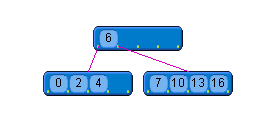
\includegraphics[width=.5\textwidth]{3.png} \\
Insert 12
\end{figure}

\begin{figure}[H]
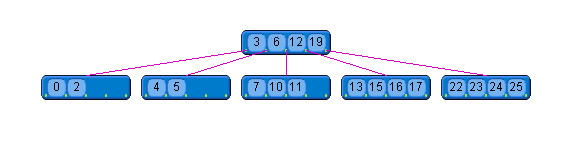
\includegraphics[width=\textwidth]{8.png}
Insert 18
\end{figure}

\begin{figure}[H]
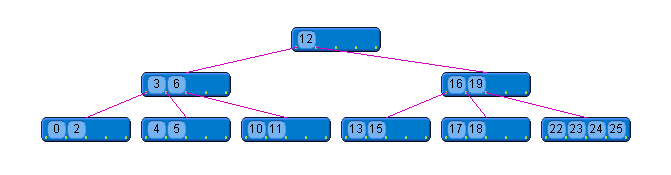
\includegraphics[width=\textwidth]{10.png}
Remove 19
\end{figure}

\begin{figure}[H]
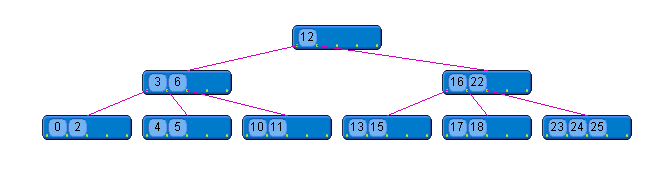
\includegraphics[width=\textwidth]{11.png}
Remove 17
\end{figure}

\begin{figure}[H]
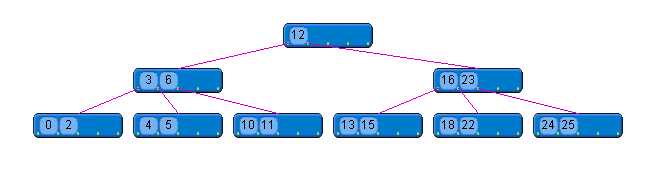
\includegraphics[width=\textwidth]{12.png}
Remove 4
\end{figure}

\end{problem}
